% porque
\chapter{Motivação}
\label{chap:estado-da-arte}

\section{Introdução}
\label{chap2:sec:intro}



% explicar que o mundo cada vez mais requer programas distribuídos devido à escalabilidade destes
% aumento de cores no CPU
% aumento da infraestruturas das grandes empresas
% A internet é cada vez mais global, logo é necessário distribuir os sistemas por várias partes do mundo
Atendendo à crescente utilização de grandes infraestruturas, como em redes sociais, grandes empresas e a demanda de maior capacidade de processamento, como por exemplo, o aumento do número de núcleos nos processadores ou a conveniência de várias máquinas trabalharem em conjunto, a necessidade do uso de sistemas distribuídos tem vindo a aumentar ao longo dos anos.
%https://www.oreilly.com/content/distributed-systems-a-quick-and-simple-definition/
% maior runtime
% fault tolearnce
% mais baratos porque escabilidade horizontal
% mais eficientes, porque é possivel várias máquinas trabalharem

Das várias vantagens no uso de sistemas distribuídos, as que mais se destacam são as seguintes.
% remover, demasiada informação desnecessária, não o ponto principal da motivação
\begin{description}
    \item [Escalabilidade Horizontal] Os sistemas distribuídos permitem que se aumente a capacidade de processamento e armazenamento ao introduzir máquinas no sistema, ao invés de melhorar uma única máquina.
	
    \item [Maior tolerância a erros]Quando o processamento está distribuído por vários nós, a falha de um único nó não levará a que o sistema num todo falhe.

    \item [Mais eficientes] O uso de algoritmos distribuídos permite um maior número de máquinas em execução concorrente, e consequentemente, a divisão do trabalho pelas várias máquinas.
	Também é possível a distribuição da localização física das máquinas, o que permite conexões de maior velocidade em outros locais no mundo.

\end{description}

No entanto, os sistemas distribuídos, que inerentemente são concorrentes, têm uma complexidade maior no desenvolvimento em comparação com sistemas e programas sequenciais.
A falta de um relógio central, a possibilidade de vários processos necessitarem de aceder ao mesmo recurso ao mesmo tempo, ordem indeterminada de quais quer pedidos, a necessidade de se usar uma rede para comunicar informação entre os nós e dificuldade de controlar os vários sistemas independentes pertencentes ao sistema distribuídos são alguns dos fatores para esta complexidade.

Um dos tópicos relacionado com o protocolo estudado neste relatório é o acesso ao mesmo recurso por vários processos.

Por exemplo, as máquinas numa rede têm a possibilidade de aceder a um ficheiro, tanto para fazer uma leitura como uma escrita.
Duas máquinas (ou processos) pretendem fazer alterações num ficheiro na rede, ambas começam por fazer uma leitura do ficheiro, e após essa leitura, uma das máquinas escreve as alterações, e logo de seguida a outra máquina escreve as alterações. A falha nesta ocorrência foi que a última máquina a escrever as alterações sobrescreveu totalmente as a alterações da primeira, visto que ambas leram o mesmo estado do ficheiro mas a uma das máquinas escreveu após a escrita da outra.

Este é um dos vários problemas do acesso não exclusivo por parte de vários processos, denominado como falha de condição de corrida/\emph{Race Condition}.

No protocolo estudado, estes problemas são evitados através da criação de uma fila, esta distribuída, que ordena/sincroniza o acesso ao objeto por parte dos vários nós do sistema.
A formação desta fila é descrita com maior pormenor na secção seguinte. 

\section{Descrição do Protocolo}

Nesta secção será descrito o funcionamento e estrutura do \textit{Arrow Distributed Directory Protocol} (\emph{Arrow}) \cite{Arrow}. 

Este sistema consiste numa rede, que permite o envio assíncrono de mensagens (ou a comunicação) entre os nós, e um diretório, que permite localizar um objeto na rede e garantir o acesso exclusivo a este. 

O diretório pode ser considerado como um grafo ou uma árvore de extensão mínima (\acs{MST}).
%%%%%%%%%%%%%%%%%%%%%%%%%%%%%%%

\begin{comment}
Rever pois isto não é bem verdade. o facto de ser “móvel” ou não depende do objecto em si, aquilo que é “móvel” pode ser simplesmente o “canal” de acesso ao objecto (imóvel). Trata-se de uma abstracção e se quiser pode explicar como tal “Consideremos que… para abstrair …” 
\end{comment}

Consideramos que o objeto é ``móvel'', no entanto esta é uma abstração do \textbf{acesso} ao objeto, e este acesso tem a possibilidade de se movimentar na rede entre os nós.

O objeto pode ser um processo, um ficheiro ou qualquer outra estrutura de dados.

Cada nó tem uma só ligação, deste para outro nó, no entanto podem existir vários nós com ligação a um único nó.

%%%%%%%%%%%%%%%%%%%%%%%%%%%%%%%

%%%%%%%%%%%%%%%%%%%%%%%%%%%%%%%
Quando um nó pretende aceder ao objeto, este envia um pedido de acesso pela sua ligação. 



Reconsideremos que a noção que o diretório é uma árvore de extensão mínima, e consideremos que o acesso ao objeto (ou o nó que o detém) está localizado na raíz da àrvore e as todas as ligações apontam em direção à raíz.

Quando é realizado um pedido, este irá chegar à raíz, pois todas as ligações apontam para esta. No final da circulação do pedido, todas as ligações por onde passou o pedido estam invertidas, para que estas passam a apontar para o nó que fez o pedido. \\

Caso um nó receba um pedido de acesso,a ligação deste passa a apontar para o nó vizinho que lhe fez chegar o pedido, ou seja, por onde passa o pedido há uma inversão do sentido da ligação.



\subsection*{Exemplo da organização das ligações}

Vejamos o seguinte exemplo da rede, em que o (acesso ao) objeto se encontra atualmente no nó \textbf{H}.

\begin{figure}[!htb]
\centering
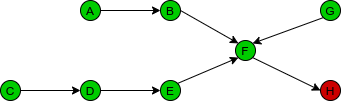
\includegraphics[width=250pt]{um_pedido_1.png}
\caption{Estado inicial do diretório}
\end{figure}

O nó \textbf{A} pretende obter o acesso ao objeto, e para tal envia um pedido através da sua ligação (para o nó \textbf{B}).
O pedido passará pelos nós \textbf{B}, \textbf{F} e \textbf{H}, por esta ordem.

Vejamos o estado após o pedido chegar ao nó \textbf{F}:

\begin{figure}[!htb]
\centering
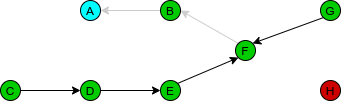
\includegraphics[width=250pt]{um_pedido_2.png}
\caption{Estado do diretório após o pedido chegar ao nó \textbf{F}}
Note que as ligações por onde o pedido do nó \textbf{A} passou inverteram-se.

\end{figure}


Quando o nó \textbf{A} faz o pedido e este chega ao \textbf{H} este passa a ser a raiz da árvore, e os seguintes pedidos serão direcionados até ao \textbf{A}.\\



Vejamos agora outro exemplo, em que exploramos o caso de existirem mais do que uma mensagem a circular no diretório:

Consideremos que cada passo é uma transmissão de pedidos entre nós, e que os passos que cada pedido executa são sincronizados com os restantes, algo que não é garantido na rede, mas que temos em conta para se demonstrar com maior simplicidade este processo.

Consideremos o mesmo estado anteriormente referido, o estado do diretório após o pedido do nó \textbf{A} chegar ao nó \textbf{F}, e que ao mesmo tempo o nó \textbf{D} pretende obter o acesso, que para tal este enviou um pedido de acesso que atualmente se encontra no nó \textbf{E}.


\begin{figure}[!htb]
\centering
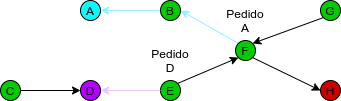
\includegraphics[width=250pt]{dois_pedidos_1.png}
\caption{Estado do diretório após o pedido do nó \textbf{A} chegar ao nó \textbf{F}, as etiquetas com ``Pedido'' indicam onde o pedido de cada nó se encontra no atual estado.}

\end{figure}

Como o nó \textbf{F} aponta/está ligado ao nó \textbf{B}, o pedido do nó \textbf{D} será então transmitido para este ao invés do \textbf{H}.
Vejamos o passo seguinte deste estado:


\begin{figure}[!htb]
\centering
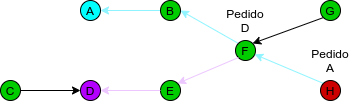
\includegraphics[width=250pt]{dois_pedidos_2.png}
\caption{Estado do diretório após o pedido do nó \textbf{D} chegar ao nó \textbf{F}}
\end{figure}

\textbf{Nota:} Caso os dois pedidos chegassem ao mesmo tempo ao nó \textbf{F}, este nó teria que decidir qual deles processar primeiro. Se o pedido do nó \textbf{A} fosse o primeiro a ser processado, este seria transmitido para o \textbf{H} e o pedido do \textbf{D} continuava a circulação em direção ao \textbf{A} e vice-versa. \\

No passo seguinte, o pedido do \textbf{D} encontra-se no nó \textbf{B}:


\begin{figure}[!htb]
\centering
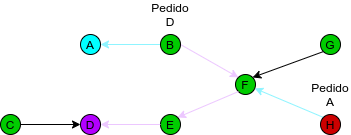
\includegraphics[width=250pt]{dois_pedidos_3.png}
\caption{Estado do diretório após o pedido do nó \textbf{D} chegar ao nó \textbf{B}}
\end{figure}

%%%%%%%%%%%%%%%%%%%%%%%%%%%%%%%

Numa vista global sobre a rede, quando um nó realiza um pedido, as ligações dos nós por onde esse pedido passou passam a indicar onde é que futuramente estará o objeto, ou seja, na direção do nó que fez o pedido e que espera pelo acesso ao objeto.
Qualquer outra ``sobreposição'' das alterações nas ligações fará com que as ligações apontem em direção dos nós que realizaram os pedidos que passaram por essas ligações, isto é, independentemente da quantidade de pedidos a circular na rede, se seguirmos as direções das ligações em qualquer estado da rede estas aponta sempre para um nó que detém ou espera pelo acesso ao objeto.

Esta inversão das ligações permite que, o nó apenas detendo uma ligação, faça chegar o seu pedido ao nó que detém o objeto ou a um nó que deterá o objeto mas que espera por ele. \\




Caso um nó que espera pelo objeto, quer porque o seu pedido ainda está em circulação na rede ou o nó detentor do objeto ainda não o cedeu, receba um pedido de acesso de outro nó, então este armazena uma ligação com o nó que realizou o pedido.

Quando o nó detém o objeto,se recebe um pedido ou tem em espera um outro nó, o objeto é cedido através de uma ligação direta entre dois nós, evitando a passagem do objeto pelo diretório.


\subsection*{Exemplo da formação de uma fila de espera}

Continuando o exemplo anterior. Vejamos um passo seguinte, em que o pedido do nó \textbf{D} chega ao nó \textbf{A}, o nó \textbf{H} ainda não cedeu o acesso ao nó \textbf{A}, e o nó \textbf{C} decidiu realizar um pedido que atualmente se encontra no nó \textbf{D}, que também está à espera do acesso ao objeto. 

\begin{figure}[!htb]
\centering
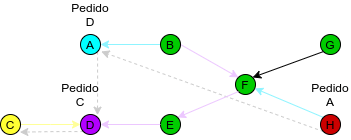
\includegraphics[width=250pt]{fila.png}
\caption{Estado do diretório com 3 pedidos em circulação.}
\textbf{Nota:} As ligações a tracejado representam as ligações entre os nós fora do diretório, usadas para a transmissão do acesso ao objeto.
\end{figure}


Temos assim os seguintes nós à espera:
\begin{enumerate}
    \item O nó \textbf{A} espera pelo nó \textbf{H}.
    \item O nó \textbf{D} espera pelo nó \textbf{A}.
    \item O nó \textbf{C} espera pelo nó \textbf{D}.
\end{enumerate}
Ou seja, a ordem de chegada e fila do acesso de pedidos será a \textbf{A},\textbf{D},\textbf{C}. \\


 

A particularidade deste protocolo deve-se à mudança tanto da localização do objeto como a sua origem, pois esta muda-se para o nó que tem o acesso ao objeto, e não há um único nó que detém a localização atual do objeto, mas a disposição de todas as ligações permite a localização do objeto por todos os nós.

O facto da origem do objeto estar em constante alteração garante que apenas um nó detenha o acesso ao objeto (acesso exclusivo), e que nenhum nó se torne num foco, isto é, que nenhum nó receba demasiados pedidos em relação a outros nós, provocado um engarrafamento/\emph{bottleneck} no acesso ao objeto.

% notas paper
% explicar o nome
% explicar que ao seguirmos as setas chegamos sempre ao objeto ou alguém que terá acesso ao mesmo
% explicar o que é um diretório
% dar uma vista global sobre
% - Objeto Movível
% O objeto move-se pelo diretório dependendo se houve pedidos por parte de Nodes

\subsection{Estrutura do Diretório}





\begin{comment}
     elementos
     - Nodes
    vértices do grafo
     

     - Ligações entre os nodes (ligação de finds e ligação do MyChan, ver ARVY)
     explicar porque é que as ligações viram
     - envios do obj são diretos
\end{comment}

\subsection{Estruturas de Dados}
Neste protocolo existem duas estruturas de dado o acesso ao objeto.

\begin{description}
    \item [Grafo] 
    \item [Fila] os vértices são todos os nós do sistema que esperam pelo acesso ao objeto (mudar porque podem haver nós que esperam mas não estão na fila) e as arestas são as ligações do tipo (tipo), pois neste circula o acesso ao objeto.
\end{description}

\section{Trabalhos relacionados}
%Ivy e Arvy
De muitos algoritmos distribuídos e suas implementações, há dois trabalhos relacionados com o protocolo estudado neste projeto. Estes são, o \emph{Ivy} \cite{Ivy} e o \emph{Arvy} \cite{Arvy}.
O \emph{Ivy} apresenta um funcionamento muito similar ao \emph{Arrow}, em que a origem do objeto muda com a posição atual deste, isto é, 



% comparar este algoritmo com outros (ver http://cs.brown.edu/people/mph/DemmerH98/disc.pdf)

% saber explicar as dificuldades da implementação do AADP (não a minha em específico, mas em geral), os seus usos e 
% porque é que é um problema relevante
% explicar benefícios da visualiazção (ponto importante, que até está no nome do AADP, as Setas)
% motivação do trabalho, porque é que é giro de se fazer
% explicar a utilidade/problemas resolvidos com este protocolo
% que problemas estamos a resolver
  % definição do problema
  % a forma como vamos resolver os problemas
% Qual é o interesse em fazer este trabalho
% quais os desafios/interesses ao fazer o projeto

\section{Conclusões}
\label{chap2:sec:concs}
